% TRABAJO DE TÍTULO
% 
% Avance Cap. 1
% 
% BERNARDO ARANCIBIA // SEBASTIÁN Machuca
% UTFSM 2010

\documentclass[letterpaper,12pt]{article}
\pdfpagewidth\paperwidth
\pdfpageheight\paperheight 
\usepackage[pdftex]{graphicx}
\usepackage[activeacute,spanish]{babel}
\usepackage{ucs}
\usepackage[utf8x]{inputenc}
\usepackage{times}
\usepackage[sc]{mathpazo}
\usepackage[colorlinks=true,linkcolor=black, urlcolor=black, citecolor=blue]{hyperref}
\usepackage[font=small,format=plain,labelfont=bf,up,up]{caption}
\fontsize{12}{12}\selectfont
\pretolerance=3000
\tolerance=3000

\title{
    \vspace*{0.5cm}
    
\includegraphics[width =0.3\textwidth]{images/utfsm.png}
    \\
        \tiny{SEDE JOSÉ MIGUEL CARRERA \\ VIÑA DEL MAR}
    \\ \vspace*{1cm}
    \Huge{"Sistema Automatizado de Ventas \\ bajo el framework Ruby on Rails"}
    \\ \large{Presentación Capítulo 1 y 2} %%%%%%%%%%%%%%%%%%%%%%%%%%%%%%
}
\author{
    Bernardo A. Arancibia Araos
        \and
        Sebastián A. Machuca Sáez
        \and 
        \vspace*{1cm}
    \textbf{Profesor Guía:} Catherine Gómez Barrera 
        \\ \vspace*{1cm}
    Técnico Universitario en Informática
}

\date{5 de Julio de 2010}

\marginparwidth 40pt
\marginparsep 10pt
\headsep .5in
    \hoffset       -1.0in  % Seteo a 0 el margen izquierdo
\oddsidemargin   3.5cm    % Margen izquierdo (pag. impar)
    \evensidemargin  0.5cm  % Alto  Legal 35,56cm
    \textwidth      15.5cm
    \topmargin      -1.5cm
    \textheight       22cm


    \long\def\@footnotetext#1{%
        \insert\footins{%
            \def\baselinestretch{1}\footnotesize
                \interlinepenalty\interfootnotelinepenalty 
                \splittopskip\footnotesep
                \splitmaxdepth \dp\strutbox \floatingpenalty \@MM
                \hsize\columnwidth \@parboxrestore
                \edef\@currentlabel{\csname p@footnote\endcsname\@thefnmark}\@makefntext
                {\rule{\z@}{\footnotesep}\ignorespaces#1\strut}%
        }%
    }

\fontsize{12}{12}\selectfont
\linespread{1.5}

\renewcommand{\labelenumi}{\alph{enumi})}
\captionsetup{figurewithin=section,tablewithin=section}

%%%%%%%%%%%%%%%%%%%% DOCUMENTO %%%%%%%%%%%%%%%%%%%%%%%%%%%%%%%%%%%%%%%%%%%%%%%%%

\begin{document}
\def\tablename{Tabla}

\maketitle %TITULO
\thispagestyle{empty}
\newpage
\tableofcontents %INDICE
\thispagestyle{empty}
\newpage
\renewcommand{\listtablename}{Índice de tablas}
\listoftables
\thispagestyle{empty}
\newpage
\listoffigures 
\thispagestyle{empty}
\newpage
%\thispagestyle{empty}
%\begin{abstract}
%\end{abstract}
%\newpage

\setcounter{page}{1}

%%%%%%%%%%%%%%%%%% INTRO %%%%%%%%%%%%%%%%%%%%%%%%%%%%%%%%%%%%%%%%%%%%%%%%%%%%%%

\setcounter{secnumdepth}{0}
\subsection{Introducción}

Desde un comienzo, los pequeños emprendedores, como lo son dueños de almacenes, minimarkets, verdulerías, entre 
otros, siempre han estado ajenos al uso de las nuevas tecnologías, ya sea porque nunca han tenido cerca una herramienta computacional 
o simplemente la han evitado todo este tiempo. A pesar de esto, ellos han sido capaces de cumplir su objetivo, vender. 

Con el paso del tiempo, gran parte de estas personas se ha dado cuenta lo difícil que 
es llevar el flujo de datos que el negocio maneja, más aún cuando hablamos de flujos que datan de 
varios años en la historia del mismo. También es importante para ellos tener una herramienta que les permita gestionar 
los datos de sus productos de forma eficiente, mediante la cual puedan centralizar la información en algún medio de 
fácil consulta y posterior modificación. Es aquí donde se ven limitados, ya que ellos no cuentan con el conocimiento necesario 
para generar algún tipo de \emph{Software}, teniendo que llevar estos flujos en cuadernos y/o hojas, los cuales inevitablemente 
se ven deteriorados con el tiempo. 

Hoy en día, \emph{Internet} es un producto que se encuentra en gran parte de los hogares en Chile, convirtiéndose en una herramienta
de fácil acceso desde cualquier parte del mundo. También todos hemos podido dar cuenta que las grandes empresas comienzan a 
hacer uso de \emph{Internet} como plataforma de negocios y de comunicación con sus clientes, con esto nace lo que conocemos como 
\emph{Web 2.0}.

Los pequeños negocios han sido marginados del avance computacional; la gran parte de los productos informáticos de 
calidad están destinados a grandes instituciones, o empresas. Por este motivo surge la motivación de realizar este proyecto, el cual 
buscará beneficiar al usuario de las herramientas computacionales de punta que hoy en día se utilizan para la gestión de compra-venta
además de brindarles una plataforma de interacción con sus clientes.



\setcounter{secnumdepth}{3}

%%%%%%%%%%%%%%%%%% CAPITULO I %%%%%%%%%%%%%%%%%%%%%%%%%%%%%%%%%%%%%%%%%%%%%%%%%%

\section{Aspectos relevantes del diseño lógico}

\subsection{Descripción de la organización}

El nombre de la organización es \emph{"Provisiones Frutas y Verduras Chusmisa"} y su dueño y administrador es el señor 
Bernardo Arancibia Quiroz. Su categoría es \emph{Pyme}, y su rubro es la \emph{venta de abarrotes}.
Su ubicación es Chusmisa \#75, Cuarto Sector El Olivar, Viña del Mar. Fue fundada el año 1995 por el mismo dueño.

El objetivo de este almacén es suministrar diferentes productos, ya sea alimenticios, de aseo general, entre otros, a los 
residentes del sector.  En la actualidad este almacén es uno de los que recibe mayor cantidad de clientes al día 
en todo el sector de El Olivar, en promedio el número de clientes es entre 300 y 400 diarios. Se destaca por su buena 
atención, además de su amplia oferta de productos.

La organización es conformada por la propia familia del dueño, quienes son también vendedores del local, estos son su 
señora y sus dos hijos.

El rol del administrador es la de recibir y encargar productos a los proveedores, a su vez la de definir el precio de 
venta de cada uno de éstos.

El rol de los vendedores se reduce solamente a vender los productos que los clientes solicitan y su reposición en las 
estanterías y refrigeradores.

El local es una casa del sector que fue adaptada para cumplir con los requisitos para ser un almacén, ya sea ampliación en 
su parte trasera para el diario vivir de la familia, y toda la parte frontal para la disposición de 
refrigeradores, congeladores, estanterías y balanzas digitales, donde se ubica físicamente el almacén. También cuenta con
Internet y un computador que en la actualidad no se utiliza con fines propios del negocio (registrar ventas, productos, etc).

Hoy en día, el negocio cuenta con una amplia gama de proveedores, entre los que se encuentran 
\emph{Coca-Cola, CCU, Savory, Ariztía, Cecinas PF, Cecinas Winter} y proveedores de verduras.
Cabe destacar que este almacén es uno de los que realiza mayores compras a la empresa \emph{Coca-Cola} en todo
Viña del Mar, lo que lo hizo acreedor de una mención importante por parte de la compañía.

\newpage

\subsection{Descripción de la situación actual}

A continuación se describirán los principales procesos que se realizan en el almacén en la actualidad: 

\begin{enumerate}
\item \textbf{Proceso de ventas:} 
Actualmente el \emph{proceso de ventas} se efectúa registrando en una máquina (pesa digital con memoria) el 
precio de cada producto que un cliente compra. Luego de registrar y/o pesar cada producto, ya sea 
unitario o a granel respectivamente, se obtiene la suma total de éstos y se escribe dicho total junto 
con la fecha en una boleta, la copia de ésta es finalmente entregada al cliente. Este es el único registro que
se tiene de las ventas realizadas. El almacén no trabaja con ningún tipo de descuento especial para los clientes.

\item \textbf{Proceso de devolución de productos:}
Ante una devolución de un determinado producto, sólo se necesita que un cliente presente su boleta y
el producto a devolver. Si el producto se encuentra en buen estado se le devuelve el dinero o si así lo quiere 
se cambia por otro producto, de lo contrario, la devolución no es efectiva. Si se desea devolver 
un producto con fecha de vencimiento, existe la posibilidad de cambiarlo por uno nuevo, si no es posible, se le 
devuelve el dinero.

\item \textbf{Proceso de compra de productos mediante crédito informal:}
Los clientes habituales tienen la posibilidad de pedir productos \emph{fiados}, los que serán 
cancelados en un futuro muchas veces no especificado. Al momento de pagar, el cliente debe
cancelar la suma total de su cuenta de \emph{fiados} o parte de ésta en efectivo. Se lleva
un listado de este tipo de ventas en un cuaderno universitario, con el nombre del cliente y el 
total de la venta respectiva, sin anotar alguna fecha.

\newpage

\item \textbf{Proceso de registro de pedidos:}
El negocio vende pan por las mañanas y las tardes, por lo que se generan largas listas de 
pedidos, sobre todo a la hora de la tarde. Existen pedidos diarios, los cuales se mantienen 
anotados en una lista. También se realizan pedidos para un solo día, o para un rango de días.

Los clientes tienen la costumbre de encargar productos contactándose vía telefónica con el 
vendedor. De esta manera, no sólo se reserva el pan, sino que también otros productos.

Todas las listas de pedidos se escriben en un cuaderno universitario, el cual se renueva cada
cierto tiempo. En este cuaderno se anota el producto pedido y nombre del cliente que realizó el 
pedido. Estos productos son reservados para cuando el cliente acuda a realizar la compra en el local. 

\item \textbf{Proceso de cálculo del libro de ventas:}
Una vez al mes se debe poner al día el \emph{Libro de Ventas}, el cual contiene un listado y 
la suma de todas las ventas realizadas por día y mes, para mantener un balance. Éste es un proceso
que demora bastante tiempo y es realizado por el mismo dueño y vendedor principal del negocio.

\item \textbf{Proceso de compra a proveedores:}
Para el abastecimiento de productos se requiere el servicio de diversos proveedores. Éstos
facilitan los productos necesarios para la venta diaria. El contacto con los proveedores se 
produce con la visita semanal de éstos para conocer el stock del negocio y ver si es necesario 
incorporar nuevos productos. Al momento de recibir un pedido desde un proveedor, se revisa la
factura para confirmar que la cantidad pedida sea la correcta. Luego de esto se archiva la factura 
junto a la de otros proveedores.

\newpage

En la actualidad existen una veintena de proveedores vinculados con el almacén, a la vez éstos entregan 
un centenar de productos a la semana, entre los que se destacan bebidas, verduras y alimentos de otro 
tipo. No existe el conocimiento de un margen de utilidad por producto.

\item \textbf{Proceso de control de stock:}
En la actualidad no existe proceso alguno que controle la cantidad de productos vendidos, devueltos o adquiridos
por el negocio.
\end{enumerate}

\newpage

\subsection{Problemas detectados}

Dados los procesos anteriormente descritos, se pudo observar que en cada uno de ellos existen los siguientes 
problemas detectados:

\begin{enumerate}
\item \textbf{Proceso de ventas:}
El dueño del negocio es quien controla los nuevos precios, esto podría generar confusión entre los vendedores dado 
que éstos podrían estar vendiendo un producto con un precio desactualizado, produciendo un error al momento 
de calcular el total de una venta.

Tampoco existe un respaldo escrito en el cual se puedan consultar
los precios para cada producto, el dueño es quien maneja los precios en su memoria. 

Otro punto muy importante que no se lleva a cabo es el control de qué productos y cuántos fueron los vendidos, con motivo de 
saber posteriormente qué producto es el más vendido, o cuál es el menos demandado, en un periodo de tiempo 
(día, mes, año), todo esto con fines netamente estadísticos.

No se realiza arqueo de caja al momento de comenzar un nuevo día de ventas.

\item \textbf{Proceso de devolución de productos:}
No existe un control acerca de los productos que son devueltos, por diversas razones, ya sea 
productos vencidos o en mal estado, o simplemente porque un cliente cometió una equivocación.

\item \textbf{Proceso de compra de productos mediante crédito informal:}
Dado el poco control de este procedimiento, muchas veces se generan problemas al momento de que un 
cliente pague una cuenta. Habitualmente ocurre que un cliente no reconoce un total que fue registrado
en algún momento del pasado. Por lo mismo, se hace necesario saber en qué fecha y qué productos fueron
los que un cliente llevó. Tampoco existe un método para cobrar algún tipo de \emph{interés} a estas cuentas.
Otro punto que no se considera es la fecha de tope que había fijado un cliente para pagar su deuda. 

Todos los registros de productos y cuentas de fiado se llevan en un cuaderno universitario, lo cual obliga 
a renovar constantemente éste, debido a su desgaste, lo que lleva consigo tener que volver a escribir 
las cuentas que no han sido canceladas.

\item \textbf{Proceso de registro de pedidos:}
Una de las ventas más importantes para este negocio es la venta del pan. Para ésta existen clientes habituales
que reservan diariamente o por un rango de días este producto (por temporada). Estos pedidos se registran en una 
lista que muchas veces no se encuentra actualizada, lo que podría generar algún encargo mal hecho.

Para encargar cualquier tipo de producto, los clientes tienen la costumbre de llamar por teléfono. En ciertas ocasiones 
el negocio se encuentra atestado de gente, por lo cual ese pedido no puede ser atendido. El registro de estos 
pedidos es mucho menos riguroso que con los pedidos del pan, ya que no se acostumbra a anotar en un medio específico 
(hoja, cuaderno, etc.).

\item \textbf{Proceso de cálculo del Libro de Ventas:}
Este proceso resulta ser demasiado tedioso, ya que no existe un medio automatizado para poder efectuar todos los 
cálculos que se necesitan.

\item \textbf{Proceso de compra a proveedores:}
El principal problema en este punto es que son los proveedores quienes poseen los datos del negocio, pero generalmente
el negocio no posee los datos de éstos, ya sea el teléfono, dirección, nombre del encargado de ventas, etc.

Otro punto importante es que el negocio al no poseer un sistema automatizado de ventas, no existe una relación directa entre 
un producto y su proveedor, por lo que si se agota el \emph{stock} de un producto es sólo el dueño del negocio quien 
conoce a quién se debe contactar para regularizar esta situación.

\newpage

\item \textbf{Proceso de control de stock:}
Al no existir un mecanismo que controle la cantidad de productos que ingresan y salen del almacén, resulta complicado llevar
un control exacto de gran parte de los anteriores procesos descritos.

\end{enumerate}

\newpage

\subsection{Descripción del sistema propuesto}

\subsubsection{Objetivos y beneficios del sistema propuesto}

\begin{description}
\item[Objetivo principal:] \mbox{} 

Construir un sistema integrado que automatice la gestión de venta, administración de productos y perfiles de usuario 
para el almacén, a la vez cumplir con el rol de \emph{Vitrina Online}, lo que consiste en un sitio web en el cual los clientes 
pueden generar pedidos y consultar los productos que se venden en el almacén junto con su precio actualizado en tiempo real.

\item[Objetivos específicos:] \mbox{}

\begin{itemize}
\item Generar y utilizar una Base de Datos que registre datos de productos, ventas, vendedores, clientes, pedidos, proveedores, entre otros.
\item Generar listado de productos, clientes y proveedores.
\item Generar informe de ventas.
\item Control de flujo de dinero, productos y pedidos.
\item Precisión en los cálculos.
\item Listar y procesar ventas por crédito informal.
\item Listar y procesar pedidos.
\item Crear una interfaz gráfica que implique un ágil proceso para los vendedores y una interfaz de
\emph{Vitrina Online} de  fácil uso para los clientes. 
\end{itemize}

\newpage

\item[Beneficios:] \mbox{} 

El sistema propuesto pretende solucionar cabalmente las debilidades del proceso de gestión
utilizado actualmente en el almacén, logrando eficiencia a través de las siguientes metas:

\begin{itemize}
\item Fácil distribución de la información.
\item Consistencia de la información entregada. 
\item Transparencia en los procesos de ventas, debido al control de productos y pedidos.
\item Posibilidad de delegar responsabilidades a nuevos vendedores, ya que existe un control en el flujo de dinero.
\item Rapidez en el proceso de ventas debido a la amistosidad de la interfaz gráfica.	
\end{itemize}

\end{description}

\newpage

\subsubsection{Descripción general de la solución propuesta}

El almacén cuenta con distintos proveedores, éstos visitan semanalmente el local para saber si es necesario reabastecer el stock de 
productos y/o  agregar nuevos productos al catálogo. Si el almacén no necesita productos de su proveedor, éste último confirmará
una nueva visita para la semana siguiente. Cuando se cumpla que el almacén necesita stock y/o ingresar un nuevo producto al 
catálogo, el proveedor generará una factura que adjuntará al momento de entregar los productos necesitados. Esta factura es 
un documento físico que no requiere digitalización por parte de la aplicación. Luego de esto se actualiza el stock de los productos que 
fueron proporcionados por el proveedor y/o se ingresará un nuevo producto a la base de datos con sus respectivos atributos, los que 
incluyen stock, proveedor, precio, etc. Con todos estos datos se podrán generar listados de proveedores con sus respectivos productos 
asociados.

Un cliente tiene dos opciones para comprar los productos existentes en el catálogo del almacén. La primera opción es ir directamente
al local para realizar la compra. La segunda opción es la de ingresar al sitio web del almacén, autentificarse como cliente y luego de
esto poder realizar su pedido. Una vez aceptado el pedido por un vendedor, el cliente debe asistir de forma presencial a concretarlo. 
Cualquiera de estas dos opciones podría implicar una compra en efectivo o una compra a crédito. Si la compra es en efectivo se 
genera un registro de la venta concretada, en el caso contrario, es decir, la compra es a \emph{Crédito Informal}, se debe verificar
la existencia del cliente en la base de datos. Si el cliente no existe en la base de datos, se procederá a ingresar sus datos como 
nuevo cliente. Una vez verificado el cliente y/o ingresado al sistema, se procederá a fijar una fecha futura de pago, la cual al 
momento de cumplirse, el cliente deberá acudir al local a pagar el total de su deuda, de lo contrario, se le cobrará un interés calculable al total 
de todas las compras hechas con crédito, luego de esto, la compra a \emph{Crédito Informal} quedará saldada, con lo cual se 
registrará finalmente como una venta concretada.

Si luego de concretada una venta, un cliente devuelve un producto, y éste está dañado o su fecha de vencimiento se ha cumplido, dicho producto se registrará como merma.

\newpage

\subsubsection{Diagrama de flujo administrativo}

El diagrama de flujo que involucra los procedimientos principales en el sistema se dividen en dos vistas:

\mbox{}
\vspace*{1cm} 
\begin{figure}[!ht]
\begin{center}
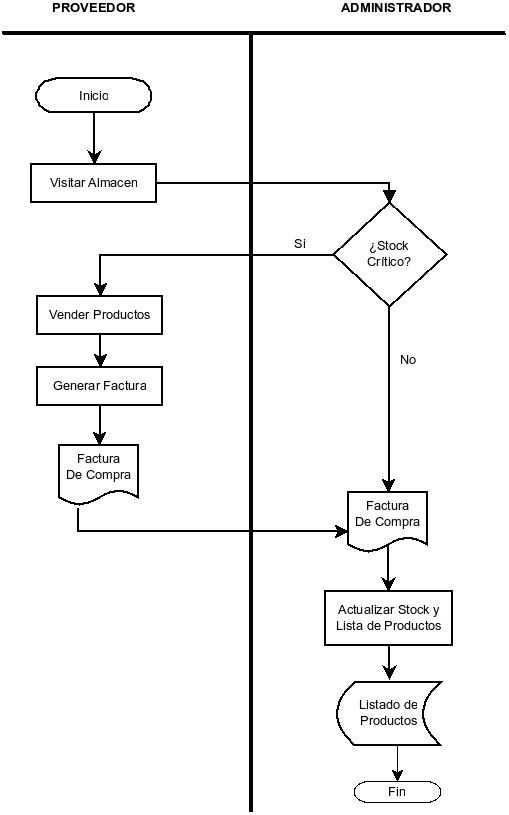
\includegraphics[width =0.62\textwidth]{images/flujoadm_proveedor_administrador.jpeg}
\end{center}
\caption{Diagrama de flujo de compra de proveedor por parte del administrador}
\end{figure}


\mbox{}
\begin{figure}[!ht]
\begin{center}
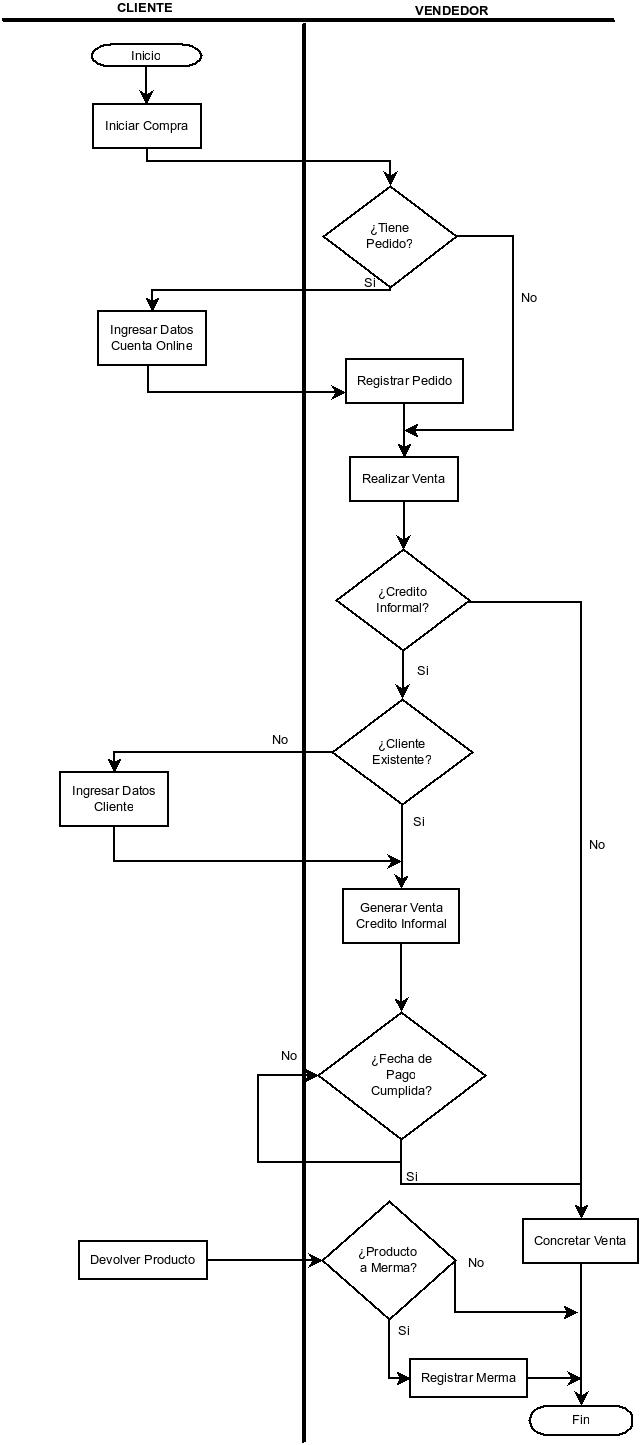
\includegraphics[width =0.5509\textwidth]{images/flujoadm_cliente_vendedor.jpeg}
\end{center}
\caption{Diagrama de flujo del proceso de venta al cliente}
\end{figure}

\newpage

\subsubsection{Estructura funcional del sistema}

A continuación se describirán las funcionalidades que contendrá el sistema a desarrollar:

\begin{enumerate} 

\item \textbf{Autenticación: }

Permite la autenticación de los distintos perfiles para ingresar al sistema.
El usuario del sistema deberá indicar si es un cliente o es un vendedor, mediante la 
aplicación. Cabe recordar que el usuario tiene contacto directo con el sistema
sólo cuando éste realiza un pedido \emph{Online}, en el caso de una compra presencial es el 
vendedor el intermediario entre el cliente y el sistema.



\item \textbf{Mantenedor de vendedores:} 



\begin{itemize}
\item \textbf{Agregar vendedor:} 
Se ingresa un nuevo vendedor a la tabla \emph{Vendedores},indicando su nombre, contraseña, algún comentario o anotación, ademas de
indicar el tipo correspondiente (administrador o usuario).

\item \textbf{Eliminar vendedor:} 
Se elimina un vendedor con sus respectivos atributos de la tabla \emph{Vendedores}, siempre que dicho 
vendedor no esté asociado a alguna venta en la tabla \emph{Ventas}.

\item \textbf{Modificar vendedor:} 
Se actualizan los atributos de un vendedor. A partir de esta funcionalidad también se podrá cambiar 
los privilegios de un determinado vendedor, es decir, cambiar los perfiles de vendedores (Administrador o Usuario).

\item \textbf{Consultar vendedor:}
Se consulta por el nombre de un vendedor.
\end{itemize}

\newpage

\item \textbf{Mantenedor de notas:}

\begin{itemize}

\item \textbf{Ingresar nota:}
Se ingresa una nota personal por cada vendedor, indicando el vendedor al que pertenece la nota, el contenido de 
la nota, la fecha y hora.

Dicha nota es un comentario o anotación (cuaderno de notas) registrada por un vendedor determinado, para 
su posterior revisión personal.

\item \textbf{Eliminar nota:}
Se eliminará físicamente una nota específica de un determinado vendedor.

\item \textbf{Modificar nota:} 
Se modificará el contenido de la nota, si así se requiere.

\item \textbf{Consultar nota:}
Un vendedor podrá listar las notas que haya realizado en una determinada fecha y hora.
Ademas, el administrador podrá consultar las notas realizadas por todos los vendedores.

\end{itemize}

\item \textbf{Mantenedor de proveedores:} 

\begin{itemize}
\item \textbf{Ingresar proveedor:}
Se ingresa un nuevo proveedor al sistema, indicando su nombre, teléfono y nombre del encargado 
de ventas de dicho proveedor.

\item \textbf{Modificar proveedor:}
Se modifican los datos de un proveedor, ya sea el nombre del proveedor, nombre del encargado de ventas del proveedor o su teléfono entre otros.

\item \textbf{Eliminar proveedor:}
Se elimina físicamente un proveedor que nunca abasteció al almacén.

\item \textbf{Consultar proveedores:}
Mostrará los datos de un proveedor indicando su nombre.
\end{itemize}

\newpage

\item \textbf{Mantenedor de clientes:} 

\begin{itemize}
\item \textbf{Ingresar cliente: }
El vendedor registra un nuevo cliente, indicando sus datos personales como es el nombre, la dirección, su teléfono , su estado 
(cliente nulo o cliente activo) y también una contraseña, con la cual el cliente podrá efectuar sus pedidos \emph{Online} en el sistema.

\item \textbf{Eliminar cliente: }
Se elimina un cliente físicamente que no tenga asociado un pedido o crédito en la base de datos del almacén.

\item \textbf{Modificar cliente: }
Se actualizan atributos de un determinado cliente, ya sea para cambiar su contraseña en caso de olvido, dirección o 
teléfono en caso de cambio. También se podrá eliminar de forma lógica un determinado cliente, modificando su estado de activo a nulo o vice versa.

\item \textbf{Consultar cliente: }
Se muestra un determinado cliente a partir de su nombre.
\end{itemize}

\item \textbf{Mantenedor de productos:}

\begin{itemize}
\item \textbf{Ingresar nuevo producto: }
Se ingresa un nuevo producto a la tabla \emph{Productos} indicando su nombre, el precio, el stock, entre otros.

\item \textbf{Eliminar un producto existente: }
Se elimina un determinado producto de la tabla \emph{Productos} que no esté asociado a un detalle de venta.

\item \textbf{Modificar un producto existente: }
Se modificarán los atributos del producto especificado, previamente validada su existencia.

\item \textbf{Consultar producto: }
Se busca un determinado producto por su nombre o categoría en la tabla \emph{Productos}.
\end{itemize}

\newpage

\item \textbf{Mantenedor de pedidos:} 

\begin{itemize}
\item \textbf{Ingresar pedido:}
Permitirá al cliente reservar una determinada lista de productos. Esta función será del tipo \emph{carrito de pedidos}, adjuntando los productos deseados como un ítem. La idea de esta aplicación es enviar este pedido a la tabla \emph{Pedidos} para reservar un determinado producto. Debe quedar en claro que esta funcionalidad no involucra el manejo de dinero (tarjetas de crédito, débito, etc.), sólo involucra el registro de los pedidos para luego ser entregados físicamente en el mismo negocio y así finalizar la transacción.     

El pedido será catalogado en dos estados:
\begin{itemize}
\item \textbf{Pedido Aceptado:} El pedido ya ha sido recepcionado por un vendedor y los productos ya han sido reservados, lo que significa que el pedido no puede ser modificado por el cliente.
\item \textbf{Pedido Pendiente:} El pedido aún no ha sido recepcionado por un vendedor, dando la oportunidad al cliente de modificar su pedido, mientras éste siga pendiente.
\end{itemize}

\item \textbf{Modificar pedido:}
El cliente puede modificar un pedido ya ingresado en el sistema mientras éste último se encuentre pendiente, es decir
no se ha concretado una venta a partir del mismo pedido. A su vez al momento de que el cliente vaya a buscar su pedido
a las instalaciones del almacén, el vendedor podrá modificar el pedido enviado, para que el cliente pueda llevar 
los productos que realmente necesita.

\item \textbf{Eliminar pedido:}
Se eliminará físicamente un determinado pedido junto con su detalle.

\item \textbf{Consultar pedidos:}
Permitirá ver todos los pedidos efectuados por los clientes.
\end{itemize}

\newpage

\item \textbf{Mantenedor de ventas:} 

\begin{itemize}
\item \textbf{Ingresar venta: }
Luego de ser concretada y pagada una venta por un cliente, se ingresará el total de la venta, su fecha y hora en la tabla 
\emph{Ventas}, a su vez se ingresa el detalle de los productos implicados en la venta en la tabla \emph{Detalles\_Ventas}. 

\item \textbf{Eliminar venta: }
Se eliminará físicamente una determinada venta junto a su detalle, accediendo a ésta mediante el número de boleta asociada a la misma venta.
Esta operación es realizada exclusivamente por el vendedor ante un posible error en el ingreso de dicha venta y no se requiera mantener un 
registro de ésta, ya que esta venta nunca fue realizada.
Antes de eliminar la venta en la base de datos, se debe actualizar el valor del stock de los productos involucrados en la venta.

\item \textbf{Modificar venta: }
Accede a una venta ya concretada para su modificación, ya sea agregar y/o eliminar uno o varios productos, de dicha venta.
Ademas se podrán diferenciar las ventas según su tipo, los tipos de ventas (campo \emph{tipo\_venta} de la tabla \emph{Ventas}) son:\begin{itemize}

\item \textbf{Venta anulada:} Eliminación lógica de una venta.

\item \textbf{Venta presencial:} Venta realizada directamente en el almacén.

\item \textbf{Pedido:} Venta realizada a través de un Pedido Online.
\end{itemize}

También permitirá modificar el tipo de pago (campo \emph{tipo\_pago} de la tabla \emph{Ventas}) de las ventas, siendo válidas las siguientes opciones:

\begin{itemize}
\item \textbf{Efectivo:} Venta ya concretada.
\item \textbf{Tarjeta de débito:} Venta pagada con tarjeta de débito.
\item \textbf{Crédito informal:} Venta aún no pagada. 
\end{itemize}


\item \textbf{Consultar venta: }
Se desplegará una determinada venta realizada por su fecha o número de boleta.

\end{itemize}


\item \textbf{Mantenedor de ventas a crédito informal:} 

\begin{itemize}
\item \textbf{Ingresar venta a crédito: }
Teniendo un cliente ya registrado, se le asigna una venta a crédito en la tabla \emph{Créditos}, para su posterior pago dada una
fecha especificada también. Con esto se modificará el tipo de pago (campo \emph{tipo\_pago} en la tabla 
        \emph{Ventas}), indicando que la venta ha sido a crédito.
Además contará con la posibilidad de aplicar un determinado interés, que se cobrará cuando la fecha de pago
sea excedida. El valor del interés se ingresará cuando se cree por primera vez una cuenta de crédito para un determinado cliente.  

\item \textbf{Modificar venta con crédito: }
En caso de error existe la posibilidad de modificar los atributos de una venta con crédito en la tabla \emph{Créditos}. 


\item \textbf{Eliminar venta con crédito: }
Permite eliminar un crédito de la tabla \emph{Créditos}.

\item \textbf{Consultar venta con crédito: }
Se mostrará una determinada venta a crédito a partir de un cliente o su fecha de 
pago.
\end{itemize}

\newpage

\item \textbf{Mantenedor de mermas:} 

\begin{itemize}
\item \textbf{Ingresar merma:}
Se registran los productos que cumplieron su fecha de vencimiento o productos devueltos en mal estado. 

El ingreso de las mermas será una cantidad de un determinado producto.

\item \textbf{Modificar merma:}
Se modifican los atributos de una merma ya ingresada.

\item \textbf{Eliminar merma:}
Se elimina un producto de la tabla \emph{Mermas} debido a un error de ingreso.

\item \textbf{Consultar mermas:}
Permite consultar por las mermas ingresadas en una determinada fecha y/o por su tipo, indicando el nombre del producto.
\end{itemize}

\item \textbf{Mantenedor de categorías:} 

\begin{itemize}
\item \textbf{Ingresar categoría:} 
Se ingresa el nombre de nueva categoría a la tabla \emph{Categorías} para poder clasificar los productos, en el caso de que el producto no tenga categoría especificada quedará la categoría ``Sin Categoría''.

\item \textbf{Modificar categoría:}
Se actualiza el nombre de una determinada categoría.

\item \textbf{Eliminar categoría:}
Se elimina una categoría que no esté asociada con un producto de la tabla \emph{Categorías}.

\item \textbf{Consultar categoría:}
Se consulta por las categorías existentes.
\end{itemize}

\newpage

\item \textbf{Generar Libro de Ventas:}
Se generará un informe del total de las ventas que se realizaron en los distintos meses del año.   
En el Libro de Ventas no se consideran las ventas que están actualmente bajo crédito, ni tampoco las ventas 
en estado de pago pendiente (pedido).

\item \textbf{Controlar devoluciones:}
Cuando se devuelve un producto se discriminará si dicho producto está en buen o mal estado.
Si el producto devuelto está en buen estado, se ajustará el stock correspondiente.
Si el producto devuelto está en mal estado, se agregará a la tabla \emph{Mermas}.

\item \textbf{Realizar arqueo de caja:}
Se indicará la cantidad de dinero con la cual se comienza y termina un día de ventas.
\end{enumerate}

\newpage

\subsubsection{Descripción de fórmulas y cálculos empleados}
A continuación se presentarán las fórmulas empleadas para la obtención de los atributos
calculables en algunas entidades:

\begin{enumerate}
\item \textbf{Total de un detalle de ventas:}
$cantidad\_producto * precio\_unitario\_producto$

\item \textbf{Total de una venta:}
$\sum{total\_detalle\_ventas}$ 

\item \textbf{Cálculo total de una venta a crédito:}
$total\_venta * valor\_interes$

\item \textbf{Total de un detalle de pedido:}
$cantidad * precio\_unitario\_producto$

\item \textbf{Total de un pedido:}
$\sum{total\_detalle\_pedido}$

\item \textbf{Total Libro de Ventas:}
$\sum{total\_ventas\_por\_mes}$

\item \textbf{Cálculo total precio producto a granel:}
$\frac{1000 * peso\_gramos\_producto}{precio\_del\_producto}$ 

\item \textbf{Cálculo de vuelto:}
$dinero\ pagado - total\_venta$

\item \textbf{Cálculo de interés de una venta a crédito:}
$valor\_interes * total\_venta + total\_venta$

\end{enumerate}

\newpage


\renewcommand{\labelenumi}{\arabic{enumi})}

\subsubsection{Entradas}

A continuación se describirán los distintos datos que se emplearán:

\begin{enumerate}
\item \textbf{Datos de proveedor:}
Nombre del proveedor, teléfono del proveedor, nombre del encargado.
\item \textbf{Datos de vendedor:}
Nombre del vendedor, contraseña del vendedor, nota del vendedor, entre otros.
\item \textbf{Datos de una nota:}
ID de la nota, ID del vendedor, contenido de la nota, fecha y hora, entre otros. 
\item \textbf{Datos de cliente:}
Nombre del cliente, contraseña del cliente, dirección del cliente y teléfono del cliente.
\item \textbf{Datos de producto:}
Nombre del producto, precio unitario, stock real, stock crítico, entre otros.
\item \textbf{Datos de categoría:}
Nombre de la categoría.
\item \textbf{Datos de crédito:} 
ID de venta, ID del cliente, fecha de pago y valor del interés.
\item \textbf{Datos de pedido:}
ID del cliente, total del pedido, id del producto (detalle del pedido), cantidad del producto (detalle del pedido), total del detalle, fecha y hora.
\item \textbf{Datos de venta:} 
ID del vendedor, total, id del producto (detalle de venta), cantidad del producto vendido (detalle de venta), total del detalle, fecha y hora, entre otros.
\item \textbf{Datos de merma:} 
ID del producto, cantidad, tipo de merma y fecha, entre otros.
\end{enumerate}

\newpage

\subsubsection{Salidas}

A continuación se describirán los distintos listados que el sistema a desarrollar presentará:

\begin{enumerate}
\item \textbf{Listado de proveedores:} 
Se listan los proveedores y sus datos asociados.

\item \textbf{Listado de vendedores:} 
Se listan los vendedores y sus datos asociados.
\item \textbf{Listado de notas por vendedor:}
Se listan las notas de un vendedor determinado.
\item \textbf{Listado de notas de todos los vendedores:}
Se listan las notas de todos los vendedores.
\item \textbf{Listado de notas por fecha y hora:}
Se listan las notas ordenadas por fecha y hora.
\item \textbf{Listado de clientes:} 
Se listan los clientes y sus datos asociados.
\item \textbf{Listado de clientes a crédito:} 
Se listan los clientes que hayan accedido a una venta por crédito informal.
\item \textbf{Listado de clientes por pedido:} 
Se listan los clientes que hayan realizado algún pedido.
\item \textbf{Listado de productos:} 
Se listan los productos y sus datos asociados.
\item \textbf{Listado de productos por tipo:} 
Se listan los productos de un tipo específico, este puede ser a Granel o Unitario.
\item \textbf{Listado de productos por stock:} 
Se listan los productos ordenados por Stock Real o Crítico.
\item \textbf{Listado de productos por categoría:} 
Se listan los productos ordenados por categoría.
\item \textbf{Listado de productos por nombre:} 
Se lista un producto determinado según su nombre.
\item \textbf{Listado de categoría:} 
Se listan las categorías disponibles.
\item \textbf{Listado de créditos:} 
Se listan las ventas a crédito informal.
\item \textbf{Informe de créditos por fecha:} 
Se listan las ventas a crédito informal en una determinada fecha.
\item \textbf{Listado de pedidos realizados:} 
Se listan los pedidos realizados.
\item \textbf{Listado de pedidos aceptados:} 
Se listan los pedidos que han sido aceptados por algún vendedor.
\item \textbf{Listado de pedidos pendientes:} 
Se listan los pedidos pendientes.
\item \textbf{Listado de ventas:} 
Se listan todas las ventas realizadas.
\item \textbf{Informe de ventas por tipo:} 
Se listan las ventas según su tipo.
\item \textbf{Informe de ventas por tipo de pago:} 
Se listan las ventas según su tipo de pago.
\item \textbf{Listado de ventas por vendedor:} 
Se listan las ventas realizadas por un vendedor determinado.
\item \textbf{Listado de ventas por fecha:} 
Se listan las ventas realizadas en una fecha determinada.
\item \textbf{Listado de mermas:} 
Se listan todas las mermas según el producto asociado.
\item \textbf{Listado de mermas por tipo:} 
Se listan las mermas según su tipo.
\item \textbf{Listado de mermas por fecha:} 
Se listan las mermas según la fecha de registro en la tabla.
\item \textbf{Informe del Libro de Ventas:} 
Se listan los totales de las ventas en un año específico.	
\item \textbf{Listado de productos más vendidos:} 
Se listan los productos más vendidos durante un periodo de tiempo específico.

\end{enumerate}

\renewcommand{\labelenumi}{\alph{enumi})}

\newpage

\subsubsection{Entidades de información}

El siguiente modelo representa las distintas relaciones entre las entidades que se involucran en el sistema:
\mbox{}
\\\vspace*{0.2cm}
\begin{figure}[!ht]
\begin{center}      
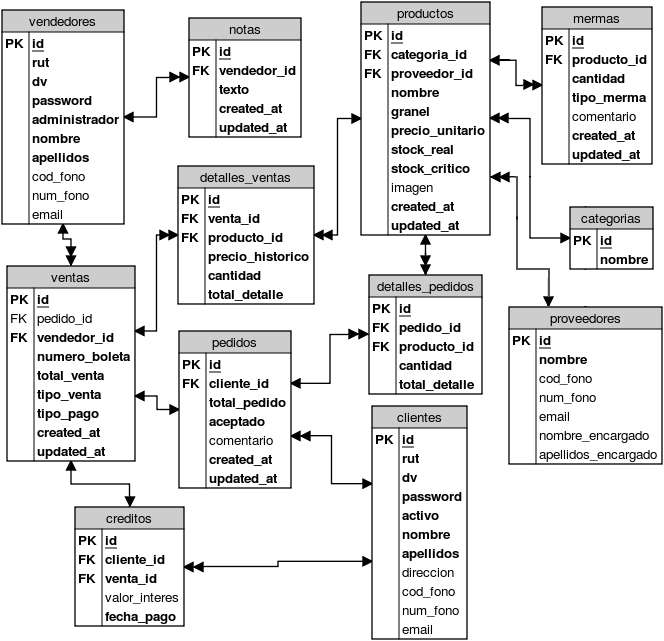
\includegraphics[width =1.0\textwidth]{images/modelo_relacional.png}
\end{center}
\caption{Modelo relacional del sistema}
\end{figure}

\newpage

\subsubsection{Estructura de códigos}

El sistema contará en su mayor parte con códigos autonuméricos, pero también existirán 
códigos que representan dos estados, a continuación se describirán los códigos utilizados:

\begin{enumerate}
\item \textbf{id:} 
autonumérico.
\item \textbf{administrador:} 
\emph{true} posee permisos de administrador, \emph{false} no posee permisos de administrador.
\item \textbf{activo:}
\emph{true} cliente activo, \emph{false} cliente inactivo.
\item \textbf{granel:}
\emph{true} a granel, \emph{false} unitario.
\item \textbf{tipo\_merma:}
0 producto con fecha de vencimiento cumplida, 1 producto dañado, 2 autoconsumo, 3 otra razón. 
\item \textbf{aceptado:}
\emph{true} pedido aceptado por el vendedor, \emph{false} pedido pendiente.
\item \textbf{tipo\_venta:}
0 venta anulada, 1 venta presencial, 2 pedido.
\item \textbf{tipo\_pago:}
0 efectivo, 1 crédito, 2 tarjeta de débito.
\end{enumerate}

\newpage

\subsubsection{Condicionantes de diseño}

En el presente proyecto se llevará a cabo un sitio web que contendrá diferentes 
funcionalidades, las que permitirán tanto el acceso, como el ingreso de datos
al mismo, haciendo uso de algunas características de la \emph{Web 2.0}. 
Esto genera distintas necesidades, como el caso de buscar un framework que se adapte 
y permita desarrollar una solución a los requisitos del cliente.

Como framework principal se hará uso de \emph{Ruby on Rails}, el cual trabaja con
la arquitectura de tres capas, \emph{Modelo, Vista y Controlador}, con lo que
se separa la \emph{presentación} de lo que se conoce como la \emph{lógica del negocio} 
en la aplicación. Gracias a estas características se podrá mantener un correcto orden de 
los distintos componentes de código del \emph{Software} a desarrollar, debido a la modularidad 
que el framework proporciona. 
Además, el lenguaje \emph{Ruby} permite desarrollar de forma natural técnicas como el manejo de la 
Orientación a Objetos, integración con Bases de Datos, Pruebas Unitarias 
(\emph{Unit Testing}), entre otras. Se hará uso de las técnicas que 
generen beneficios tanto en la etapa de desarrollo como en la implementación; 
que éste sea de calidad y que cumpla, a la vez, con las necesidades propuestas 
por el futuro usuario de la aplicación.

La política de respaldo de información con la que se trabajará será a través de las funciones que
provee el servidor de \emph{Hosting}, el cual permite realizar un \emph{pull}\footnote{Obtención de los datos.} de la 
base de datos del servidor hacia el computador local, o en su defecto un \emph{push}\footnote{Envío de los datos.} de los datos de la 
base de datos local hacia el servidor. Con esto se podrá trabajar tanto en el sitio 
web del almacén como a nivel local, con una copia del sitio completo en el \emph{localhost}, si es que no se tuviese Internet 
disponible, para luego hacer la correspondiente actualización de los datos con los mecanismos mencionados.

\newpage

%%% CAPITULO 2 %%%

\section{Medio ambiente computacional y descripción de archivos}

\subsection{Características del recurso computacional}

\subsubsection{Configuración del sistema}

A continuación se presentarán los equipos computacionales que se verán involucrados, tanto para 
conformar el sistema funcional a implementar, como los equipos que permiten su desarrollo. También 
se describirán los requisitos mínimos de los equipos para poder acceder al sistema de forma externa.

\begin{enumerate}

\item \textbf{Hosting básico Heroku}

\begin{itemize}
\item \textbf{Espacio base de datos:}
5 MB gratuitos.
\item \textbf{Espacio archivos:}
100 MB gratuitos.
\end{itemize}

Existe la posibilidad de ampliar el tamaño de almacenamiento por parte del \emph{Hosting} con un costo de 
USD \$15. Se considerará utilizar el \emph{Hosting básico gratuito} para la implementación ya que el flujo de datos 
no requiere mayor almacenamiento. 

\item \textbf{Equipo cliente local}

\begin{itemize}

\item \textbf{Tipo: }
Desktop.
\item \textbf{Procesador: }
AMD Athlon XP 2000+ (1,8 GHZ).
\item \textbf{Almacenamiento primario: }
Disco Duro Maxtor 20 GB (ATA).
\item \textbf{Almacenamiento secundario: }
Memoria Ram Kingston DDR 400 MHz 512 MB.
\item \textbf{Mecanismo de respaldo: }
Servidor externo \emph{Heroku}.
\item \textbf{Pantalla: }
Monitor CRT 15".
\end{itemize}

\newpage

\item \textbf{Equipo de desarrollo 1}

\begin{itemize}
\item \textbf{Tipo: }
Notebook Acer Aspire 4535.
\item \textbf{Procesador: }
AMD Turion X2 (2,1 GHZ).
\item \textbf{Almacenamiento primario: }
Disco Duro Hitachi 320 GB (SATA).
\item \textbf{Almacenamiento secundario: }
Memoria Ram Kingston 3 GB.
\item \textbf{Pantalla: }
LCD 14".
\end{itemize}

\item \textbf{Equipo de desarrollo 2}

\begin{itemize}
\item \textbf{Tipo: }
Notebook Dell Inspiron 1420.
\item \textbf{Procesador: }
Intel Core 2 Duo (1,6 GHZ) .
\item \textbf{Almacenamiento primario: }
Disco Duro Hitachi 120 GB (SATA).
\item \textbf{Almacenamiento secundario: }
Memoria Ram Kingston 2 GB.
\item \textbf{Pantalla: }
LCD 14".
\end{itemize}

\item \textbf{Requisitos mínimos equipo cliente externo}

\begin{itemize}
\item \textbf{Procesador:}
Procesador genérico, 500 Mhz o superior.

\item \textbf{Almacenamiento primario:}
Disco Duro 100 MB o superior.

\item \textbf{Almacenamiento secundario:}
Memoria Ram 256 MB o superior.

\item \textbf{Conexión a Internet:}
512 Kbps o superior.

\item \textbf{Navegador Web:}
Mozilla Firefox, Opera, Chrome, Safari, Internet Explorer, con soporte de 
\emph{Javascript}.
\end{itemize}

\end{enumerate}

\newpage

\subsubsection{Software utilizado}

\begin{itemize}
\item \textbf{Sistema Operativo} \\
El Sistema Operativo que utilizarán los equipos de desarrollo e implementación será \emph{GNU/Linux}. 
La razón de ésto es su alta seguridad y estabilidad, la integración del \emph{framework Ruby on Rails} 
con la consola de comandos que proporciona el sistema, esto último permite una forma más cómoda y rápida 
de manejar el ambiente interno de la aplicación \footnote{Base de datos, instancias de los modelos (MVC), manejo de archivos, etc.}
sin tener que pasar por los formularios web (en la etapa de desarrollo). La elección de la distribución \emph{Debian Linux} se basa en 
que ésta reune el conjunto de software más estable y probada entre todas las distribuciones \emph{Linux} del momento, un 
cambio a cualquiera de las otras distribuciones disponibles no supone una mayor diferencia.

\begin{enumerate}
\item \textbf{Equipo cliente:}
Debian GNU/Linux 
\item \textbf{Equipo de desarrollo 1:}
Open Suse GNU/Linux, versión 11.2.
\item \textbf{Equipo de desarrollo 2:}
Archlinux GNU/Linux, versión 2010.
\end{enumerate}

\newpage

\item \textbf{Herramientas de desarrollo de Software}

\begin{enumerate}
\item \textbf{Ruby on Rails:}
Esta es la principal herramienta a utilizar. Es un \emph{framework}, libre y multiplataforma, para el desarrollo web que
hace uso del lenguaje de programación \emph{Ruby} y el patrón de diseño \emph{Modelo, Vista y
Controlador} (MVC). Dentro de este \emph{framework}, se puede encontrar una infinidad de herramientas 
como es el caso de \emph{helpers y validadores} que permiten la integración del lenguaje de programación 
propio con el código \emph{HTML}, generando un archivo con la extensión \emph{"html.erb"}. 

\emph{Rails} \footnote{El framework Ruby on Rails tiene distintas acepciones, como lo son Rails, RoR, entre otras.} 
está focalizado en el desarrollo de aplicaciones web que hacen uso de bases de datos para mantener la persistencia 
de los datos que se involucran en el sistema.

El \emph{Modelo} es el componente encargado del acceso a la capa de almacenamiento de datos (base de datos), en éste se definen 
las entidades de información que contiene el sistema, además de definir las reglas del negocio (funcionalidades del sistema). 
La \emph{Vista} define la interfaz de usuario a través de formularios indicados para interactuar con la aplicación 
(generalmente \emph{HTML, Javascript, CSS}). Finalmente el \emph{Controlador} recibe los eventos de entrada (un click, envío de datos 
desde un formulario, etc.) y los gestiona; estas acciones pueden suponer peticiones al modelo o a las vistas. 

Para el manejo y acceso de la base de datos, se utilizará el partón de diseño conocido como \emph{ActiveRecord}. Este patrón de diseño
permite crear un \emph{Objeto} el cual \emph{envuelve} una tabla \emph{SQL}, agregándole la lógica del modelo y el control de acceso.
Esto también es conocido como \emph{Mapeo Objeto Relacional (ORM\footnote{Por sus siglas en inglés Object Relational Mapping})}.

\newpage

\emph{ActiveRecord} permite unir dos mundos totalmente diferentes, la \emph{Programación Orientada a Objetos 
(OOP\footnote{Por sus siglas en inglés Object Oriented Programming.})} que es un mundo intuitivo y natural, con el mundo 
rígido de los datos relacionales (\emph{SQL}).

\emph{Ruby on Rails} es el \emph{framework} insignia de la \emph{Metodología de Desarrollo Ágil}, ya que está focalizado 
en el desarrollo rápido, intuitivo, junto con la menor \emph{redundancia de código}\footnote{DRY: No repetir código, reutilizarlo como 
si fuesen módulos.}. Éste fue el precursor de este tipo de desarrollo, con lo que motivó el surgimiento de otras alternativas que hacen 
uso de la idea de \emph{Rails} como es el caso de los \emph{frameworks} \emph{Symfony}, \emph{CakePHP}, \emph{Django}, \emph{Merb}, \emph{Spring
Roo}, \emph{Grails}, entre muchos otros.

\newpage

\item \textbf{PostgreSQL:}
Es un motor de base de datos (DBMS) relacionales y uno de los principales representantes del \emph{Software Libre}.
Se destaca por su escalabilidad en comparación con alternativas libres como \emph{Mysql}. 

Como muchos otros proyectos de código abierto, el desarrollo de \emph{PostgreSQL} no es manejado por una sola empresa, sino 
que es dirigido por una comunidad de desarrolladores y organizaciones comerciales las cuales trabajan en su desarrollo.
Dicha comunidad es denominada el PGDG (\emph{PostgreSQL Global Development Group}).

\item \textbf{JQuery:}
Es una biblioteca o \emph{framework} de \emph{Javascript} que facilita la integración del lenguaje con \emph{HTML}.
Permite la manipulación del \emph{árbol DOM}\footnote{Interfaz de programación de aplicaciones 
que proporciona un conjunto estándar de objetos para representar documentos HTML y XML, una interfaz estándar 
para acceder a ellos y manipularlos.}, manejar 
eventos, realizar animaciones y soporte con tecnologías como \emph{AJAX}.

\item \textbf{GIT:}
Es un sistema distribuido de \emph{Control de Versiones} desarrollado por \emph{Linus Torvalds}, el creador del 
\emph{kernel Linux}. Consta de un directorio de trabajo local, el cual se sincroniza con un repositorio remoto, que mantiene  
el historial de los cambios realizados en el código del \emph{Software} a desarrollar. Permite gestionar las distintas 
versiones con \emph{flags} (ej. \emph{version 1.2.3}), retroceder a versiones anteriores, trabajo con múltiples desarrolladores, 
entre otras muchas funciones.

\item \textbf{Gema Heroku:} Herramienta desarrollada en el lenguaje \emph{Ruby}, la cual permite implementar de 
forma muy sencilla y haciendo uso de \emph{GIT} la aplicación final escrita en \emph{Ruby on Rails}. Una \emph{gema}
es un módulo o librería escrita en \emph{Ruby}.

Otra característica importante de esta herramienta es el manejo de la información que contiene la base de datos involucrada 
en el sistema, mediante ésta se podrá migrar los datos desde el cliente hacia el servidor o viceversa. 

\item \textbf{VIM:} 
Es un editor de texto por consola, que mediante a \emph{plugins} y configuraciones desarrollados por el mismo usuario, permiten 
convertirlo finalmente en un IDE completo para el desarrollo, en este caso, de aplicaciones \emph{Rails}.
\end{enumerate}



\item \textbf{Lenguaje de comandos}
\begin{enumerate}
\item \textbf{Bash:}
Lenguaje básico de los sistemas \emph{Unix}. Se utilizarán comandos de sistema para realizar ciertas tareas que lo 
impliquen, como es el caso de automatizaciones (\emph{crontab}) de respaldo de datos cliente-servidor (\emph{Gema Heroku}), entre otras.

\item \textbf{Consola Rails:} \emph{Ruby on Rails} proporciona una consola que permite trabajar con todo el sistema
desarrollado, ya sea con los modelos creados (MVC), crear instancias de éstos; acceso a la base de datos, entre otras.
\end{enumerate}
\end{itemize}

\newpage

\subsection{Descripción de archivos}

%\begin{itemize}

%\item \textbf{Listado de Tablas} \\ \mbox{}
\subsubsection{Listado de Tablas}
A continuación se listarán todas las tablas involucradas en el sistema.
\begin{enumerate}
\item \textbf{Vendedores:} Guarda datos de los vendedores.
\item \textbf{Clientes:} Guarda datos de los clientes.
\item \textbf{Proveedores:} Guarda datos de los proveedores.
\item \textbf{Productos:} Guarda datos de los productos.
\item \textbf{Categorías:} Guarda datos de las categorías asociadas a los productos.
\item \textbf{Ventas:} Guarda datos de las ventas realizadas.
\item \textbf{Detalles Ventas:} Guarda el detalle de una venta realizada.
\item \textbf{Pedidos:} Guarda datos de un pedido realizado por un cliente.
\item \textbf{Detalles Pedidos:} Guarda el detalle de un pedido realizado por un cliente.
\item \textbf{Créditos:} Guarda datos de una venta a crédito informal.
\item \textbf{Mermas:} Guarda datos de las mermas de productos.
\item \textbf{Notas:} Guarda las anotaciones personales de un vendedor determinado.
\end{enumerate}

\newpage

\subsubsection{Descripción detallada de tablas}

Se utilizarán los siguientes tipos de datos que provee PostgeSQL.

\begin{table}[!ht]
\caption{Tipos de datos en PostgeSQL}
\begin{center}
\begin{tabular}{|l|l|}
\hline
\textbf{Nombre} & \textbf{Descripción} \\ 
\hline
smallint & desde -32768 hasta +32767\\
\hline
integer & desde -9223372036854775808 hasta 9223372036854775807\\
\hline
real & Precisión 6 decimales\\
\hline
boolean & 1 ó 0, TRUE ó FALSE, t ó f, yes ó no\\
\hline
character & Cadena de caracteres largo dinámico\\
varying &\\
\hline
text & Texto ilimitado\\
\hline
date & Fecha aaaa-mm-dd\\
\hline
timestamp & Fecha y Hora aaaa-mm-dd hh:mm:ss\\
\hline

\end{tabular}
\end{center}
\end{table}

\newpage

\begin{enumerate}
%\begin{itemize}
\item \textbf{\underline{Tabla Vendedores}}
\begin{itemize}
\item \textbf{Nombre lógico:} Vendedores.
\item \textbf{Nombre físico:} vendedores.
\item \textbf{Descripción:} Esta tabla almacenará la información de todos los vendedores del almacén y sus distintos perfiles.
\item \textbf{Clave primaria:} id.
\item \textbf{Descripción de Campos:}
\end{itemize}
%\end{itemize}

\begin{table}[!ht]
\caption{Campos tabla Vendedores}
\begin{center}
\begin{tabular}{|l|l|l|l|}
\hline
\textbf{Campo} \hspace*{2cm} & \textbf{Tipo} & \textbf{Tamaño/Largo} & \textbf{Descripción} \hspace*{3cm} \\
\hline
id & integer & 4 bytes& Número que identifica\\ 
\mbox{} & \mbox{} & & de forma única \\
\mbox{} & \mbox{} & & a un vendedor en el sistema.\\
\hline
rut & integer & 4 bytes & Contiene el RUT\\
\mbox{} & \mbox{} & & sin dígito verificador,\\
\mbox{} & \mbox{} & & nombre de usuario para\\
\mbox{} & \mbox{} & & acceder a la aplicación.\\
\hline
dv & character & 1 character& Contiene el Dígito Verificador\\
\mbox{} & varying & & del RUT.\\
\hline
password & character & 15 caracteres & Contiene contraseña.\\
\mbox{} & varying & & del vendedor para acceso\\
\mbox{} & \mbox{} & & a la aplicación.\\
\hline

\end{tabular}
\end{center}
\end{table}


\newpage
\begin{table}[!ht]
\begin{center}
\begin{tabular}{|l|l|l|l|}
\hline
\textbf{Campo} \hspace*{2cm} & \textbf{Tipo} & \textbf{Tamaño/Largo} & \textbf{Descripción} \hspace*{3,5cm} \\
\hline

administrador & boolean & 4 bytes & Contiene el tipo\\
\mbox{} & \mbox{} & & de vendedor, indica\\
\mbox{} & \mbox{} & & administrador (true), \\
\mbox{} & \mbox{} & & vendedor (false). \\
\hline
nombre & character & 30 caracteres & Contiene el nombre\\
\mbox{} & varying & & del vendedor. \\

\hline
apellidos & character & 30 caracteres & Contiene los apellidos\\
\mbox{} & varying & & del vendedor. \\
\hline

cod\_fono & smallint & 2 bytes & Contiene el código\\
\mbox{} & \mbox{} & & de área del\\
\mbox{} & \mbox{} & & teléfono del vendedor.\\
\hline
num\_fono & smallint & 2 bytes & Contiene el número\\
\mbox{} & \mbox{} & & del teléfono del vendedor.\\
\hline
email & character & 255 caracteres & Contiene el correo\\
\mbox{} & varying & & electrónico del vendedor.\\
\hline

\end{tabular}
\end{center}
\end{table}

\newpage

%\begin{itemize}
\item \textbf{\underline{Tabla Clientes}}
\begin{itemize}
\item \textbf{Nombre lógico:} Clientes.
\item \textbf{Nombre físico:} clientes.
\item \textbf{Descripción:} Esta tabla almacenará la información de todos los clientes registrados en el almacén.
\item \textbf{Clave primaria:} id.
\item \textbf{Descripción de Campos:}
\end{itemize}
%\end{itemize}

\begin{table}[!ht]
\caption{Campos tabla Clientes}
\begin{center}
\begin{tabular}{|l|l|l|l|}
\hline
\textbf{Campo} \hspace*{2cm} & \textbf{Tipo} & \textbf{Tamaño/Largo} & \textbf{Descripción} \hspace*{3,5cm} \\
\hline
id & integer & 4 bytes & Número que identifica\\ 
\mbox{} & \mbox{} & & de forma única \\
\mbox{} & \mbox{} & & a un cliente en el sistema.\\
\hline

rut & integer & 4 bytes & Contiene el RUT\\
\mbox{} & \mbox{} & & sin dígito verificador,\\
\mbox{} & \mbox{} & & que será utilizado para\\
\mbox{} & \mbox{} & & acceder a la aplicación.\\
\hline
dv & character & 1 caracter& Contiene el Dígito Verificador\\
\mbox{} & varying & & del RUT.\\
\hline

password & character & 15 caracteres & Contiene contraseña.\\
\mbox{} & varying & & del cliente para acceso\\
\mbox{} & \mbox{} & & a la aplicación.\\
\hline

\end{tabular}
\end{center}
\end{table}


\newpage
\begin{table}[!ht]
\begin{center}
\begin{tabular}{|l|l|l|l|}
\hline
\textbf{Campo} \hspace*{2cm} & \textbf{Tipo} & \textbf{Tamaño/Largo} & \textbf{Descripción} \hspace*{3,5cm} \\
\hline

activo & boolean & 4 bytes & Contiene el estado\\
\mbox{} & \mbox{} & & del cliente, indica\\
\mbox{} & \mbox{} & & activo (true), \\
\mbox{} & \mbox{} & & inactivo (false). \\
\hline
nombre & character & 30 caracteres & Contiene el nombre\\
\mbox{} & varying & & del cliente. \\

\hline
apellidos & character & 30 caracteres & Contiene los apellidos\\
\mbox{} & varying & & del cliente. \\
\hline
direccion & character & 30 caracteres & Contiene la dirección\\
\mbox{} & varying & & del cliente.\\
\hline

cod\_fono & smallint & 2 bytes & Contiene el código\\
\mbox{} & \mbox{} & & de área del\\
\mbox{} & \mbox{} & & teléfono del cliente.\\
\hline
num\_fono & smallint & 2 bytes & Contiene el número\\
\mbox{} & \mbox{} & & del teléfono del cliente.\\
\hline
email & character & 255 caracteres & Contiene el correo\\
\mbox{} & varying & & electrónico del cliente.\\
\hline



\end{tabular}
\end{center}
\end{table}



\newpage

%\begin{itemize}
\item \textbf{\underline{Tabla Proveedores}}
\begin{itemize}
\item \textbf{Nombre lógico:} Proveedores.
\item \textbf{Nombre físico:} proveedores.
\item \textbf{Descripción:} Esta tabla almacenará la información de todos los proveedores que abastecen al almacén.
\item \textbf{Clave primaria:} id.
\item \textbf{Descripción de Campos:}
\end{itemize}
%\end{itemize}

\begin{table}[!ht]
\caption{Campos tabla Proveedores}
\begin{center}
\begin{tabular}{|l|l|l|l|}
\hline
\textbf{Campo} \hspace*{2cm} & \textbf{Tipo} & \textbf{Tamaño/Largo} & \textbf{Descripción} \hspace*{3,5cm} \\
\hline
id & integer & 4 bytes&Número que identifica\\ 
\mbox{} & \mbox{} & &de forma única a un\\
\mbox{} & \mbox{} & &proveedor en el sistema.\\
\hline

nombre & character & 30 caracteres&Contiene nombre\\
\mbox{} & varying & &del proveedor.\\
\hline
cod\_fono & smallint & 2 bytes & Contiene el código\\
\mbox{} & \mbox{} & & de área del\\
\mbox{} & \mbox{} & & teléfono del proveedor.\\
\hline
num\_fono & smallint & 2 bytes & Contiene el número\\
\mbox{} & \mbox{} & & del teléfono del proveedor.\\
\hline
email & character & 255 caracteres& Contiene el correo\\
\mbox{} & varying & & electrónico del proveedor.\\
\hline
\end{tabular}
\end{center}
\end{table}

\newpage

\begin{table}[!ht]
\begin{center}
\begin{tabular}{|l|l|l|l|}
\hline
\textbf{Campo} \hspace*{2cm} & \textbf{Tipo} & \textbf{Tamaño/Largo} & \textbf{Descripción} \hspace*{3,5cm} \\
\hline

nombre\_encargado & character & 30 caracteres&Contiene nombre\\
\mbox{} & varying & &del encargado de\\
\mbox{} & \mbox{} & &ventas del proveedor.\\
\hline
apellidos\_encargado & character & 30 caracteres&Contiene apellidos\\
\mbox{} & varying & &del encargado de\\
\mbox{} & \mbox{} & &ventas del proveedor.\\
\hline


\end{tabular}
\end{center}
\end{table}

\newpage

%\begin{itemize}
\item \textbf{\underline{Tabla Productos}}
\begin{itemize}
\item \textbf{Nombre lógico:} Productos.
\item \textbf{Nombre físico:} productos.
\item \textbf{Descripción:} Esta tabla almacenará la información de todos los productos disponibles a la venta en el almacén.
\item \textbf{Clave primaria:} id.
\item \textbf{Claves foráneas:} proveedor\_id referencia a tabla \emph{Proveedores}, categoria\_id referencia a tabla \emph{Categorías}.
\item\textbf{Descripción de Campos:}
\end{itemize}
%\end{itemize}

\begin{table}[!ht]
\caption{Campos tabla Productos}
\begin{center}
\begin{tabular}{|l|l|l|l|}
\hline
\textbf{Campo} \hspace*{2cm} & \textbf{Tipo} & \textbf{Tamaño/Largo} & \textbf{Descripción} \hspace*{3,5cm} \\
\hline
id & integer & 4 bytes&Número que identifica de forma\\ 
\mbox{} & \mbox{} & &única a un producto en el sistema.\\
\hline

categoria\_id & integer & 4 bytes&Contiene id de la categoría\\
\mbox{} & \mbox{} & &del producto.\\
\hline

proveedor\_id & integer & 4 bytes&Contiene id del proveedor\\
\mbox{} & \mbox{} & &que suministra el producto.\\
\hline

nombre & character & 30 caracteres&Contiene nombre del producto.\\
& varying & & \\
\hline

\end{tabular}
\end{center}
\end{table}

\newpage

\begin{table}[!ht]
\begin{center}
\begin{tabular}{|l|l|l|l|}
\hline
\textbf{Campo} \hspace*{2cm} & \textbf{Tipo} & \textbf{Tamaño/Largo} & \textbf{Descripción} \hspace*{3,5cm} \\
\hline

granel & boolean & 4 bytes &Contiene tipo del producto,\\
\mbox{} & \mbox{} & &a granel (true)\\
\mbox{} & \mbox{} & &o unitario (false).\\
\hline


precio\_unitario & integer &4 bytes &Contiene precio por unidad o Kg.\\
\hline

stock\_real & smallint &2 bytes &Contiene valor de stock\\
\mbox{} & \mbox{} & &de un producto. \\
\hline

stock\_critico & smallint &2 bytes &Contiene valor mínimo de stock\\
\mbox{} & \mbox{} & &que admite el almacén para\\
\mbox{} & \mbox{} & &un producto. \\
\hline

imagen & character &30 caracteres &Contiene nombre de la imagen \\
\mbox{} & varying & &asociada a un producto,\\
\mbox{} & \mbox{} & &la cual será concatenada junto\\
\mbox{} & \mbox{} & &a la ruta donde se almacenan\\
\mbox{} & \mbox{} & &las imágenes.\\
\hline

created\_at& timestamp & 8 bytes &Contiene fecha y hora\\
\mbox{} & \mbox{} & &de la creación del producto.\\
\hline
updated\_at& timestamp & 8 bytes &Contiene fecha y hora \\
\mbox{} & \mbox{} & &de la última actualización\\
\mbox{} & \mbox{} & &del producto.\\
\hline

\end{tabular}
\end{center}
\end{table}


\newpage

%\begin{itemize}
\item \textbf{\underline{Tabla Categorías}}
\begin{itemize}
\item \textbf{Nombre lógico:} Categorías.
\item \textbf{Nombre físico:} categorias.
\item \textbf{Descripción:} Esta tabla almacenará la información de las categorías disponibles para clasificar los productos.
\item \textbf{Clave primaria:} id.
\item\textbf{Descripción de Campos:}
\end{itemize}
%\end{itemize}

\begin{table}[!ht]
\caption{Campos tabla Categorías}
\begin{center}
\begin{tabular}{|l|l|l|l|}
\hline
\textbf{Campo} \hspace*{2cm} & \textbf{Tipo} & \textbf{Tamaño/Largo} & \textbf{Descripción} \hspace*{3,5cm} \\
\hline

id& integer & 4 bytes&Contiene id de la categoría\\
\mbox{} & \mbox{} & &del producto.\\
\hline

nombre & character & 30 caracteres&Contiene nombre de la categoría.\\
& varying & & \\
\hline

\end{tabular}
\end{center}
\end{table}

\newpage

%\begin{itemize}
\item \textbf{\underline{Tabla Ventas}}
\begin{itemize}
\item \textbf{Nombre lógico:} Ventas.
\item \textbf{Nombre físico:} ventas.
\item \textbf{Descripción:} Esta tabla almacenará la información de todas las ventas realizadas en el almacén.
\item \textbf{Clave primaria:} id.
\item \textbf{Claves foráneas:} pedido\_id referencia a tabla \emph{Pedidos}, vendedor\_id referencia a tabla \emph{Vendedores}.
\item\textbf{Descripción de Campos:}
\end{itemize}
%\end{itemize}

\begin{table}[!ht]
\caption{Campos tabla Ventas}
\begin{center}
\begin{tabular}{|l|l|l|l|}
\hline
\textbf{Campo} \hspace*{2cm} & \textbf{Tipo} & \textbf{Tamaño/Largo} & \textbf{Descripción} \hspace*{3,5cm} \\
\hline
id & integer & 4 bytes&Número que identifica de forma\\ 
\mbox{} & \mbox{} & &única a una venta en el sistema.\\
\hline

pedido\_id & integer & 4 bytes&Contiene id de un\\
\mbox{} & \mbox{} & &pedido asociado.\\
\hline

vendedor\_id & integer & 4 bytes&Contiene id del vendedor\\
\mbox{} & \mbox{} & &que realiza la venta.\\
\hline

numero\_boleta & integer & 4 bytes&Contiene numero de boleta.\\
\hline

total\_venta & integer & 4 bytes&Contiene total de la\\
\mbox{} & \mbox{} & &venta realizada.\\
\hline

tipo\_venta & character &1 caracter &Contiene tipo de la venta, \\
\mbox{} & varying & &anulada (valor 0),\\
\mbox{} & \mbox{} & &presencial (valor 1)\\
\mbox{} & \mbox{} & &o pedido (valor 2).\\

\hline

\end{tabular}
\end{center}
\end{table}

\newpage

\vspace*{-1cm}
\begin{center}
\begin{table}
\begin{tabular}{|l|l|l|l|}
\hline
\textbf{Campo} \hspace*{2cm} & \textbf{Tipo} & \textbf{Tamaño/Largo} & \textbf{Descripción} \hspace*{3,5cm} \\
\hline

tipo\_pago & character &1 caracter &Contiene tipo de pago, \\
\mbox{} & varying & &efectivo (valor 0),\\
\mbox{} & \mbox{} & &crédito (valor 1)\\
\mbox{} & \mbox{} & &o tarjeta (valor 2).\\

\hline
created\_at& timestamp & 8 bytes &Contiene fecha y hora\\
\mbox{} & \mbox{} & &de la creación de la venta.\\
\hline
updated\_at& timestamp & 8 bytes &Contiene fecha y hora\\
\mbox{} & \mbox{} & &de la última actualización\\
\mbox{} & \mbox{} & &de la venta.\\
\hline

\end{tabular}

\end{table}

\end{center}

\newpage

\item \textbf{\underline{Tabla Detalle Ventas}}
\begin{itemize}
\item \textbf{Nombre lógico:} Detalle Ventas.
\item \textbf{Nombre físico:} detalle\_ventas.
\item \textbf{Descripción:} Esta tabla almacenará la información del detalle de una venta.
\item \textbf{Clave primaria:} id.
\item \textbf{Claves foráneas:} producto\_id referencia a tabla \emph{Productos}, venta\_id referencia a tabla \emph{Ventas}.
\item\textbf{Descripción de Campos:}
\end{itemize}

\begin{table}[!ht]
\caption{Campos tabla Detalle Ventas}
\begin{center}
\begin{tabular}{|l|l|l|l|}
\hline
\textbf{Campo} \hspace*{2cm} & \textbf{Tipo} & \textbf{Tamaño/Largo} & \textbf{Descripción} \hspace*{3,5cm} \\
\hline
id & integer & 4 bytes&Número que identifica \\ 
\mbox{} & \mbox{} & &a una linea de detalle.\\
\hline

venta\_id & integer & 4 bytes&Contiene id de una\\
\mbox{} & \mbox{} & &venta asociada.\\
\hline

producto\_id & integer & 4 bytes&Contiene id del producto\\
\mbox{} & \mbox{} & &involucrado en la venta.\\
\hline

\end{tabular}
\end{center}
\end{table}

\newpage
\begin{table}[!ht]
\begin{center}
\begin{tabular}{|l|l|l|l|}
\hline
\textbf{Campo} \hspace*{2cm} & \textbf{Tipo} & \textbf{Tamaño/Largo} & \textbf{Descripción} \hspace*{3,5cm} \\
\hline

precio\_historico & integer & 4 bytes&Contiene el precio que el\\
\mbox{} & \mbox{} & &producto tuvo al momento\\
\mbox{} & \mbox{} & &de su compra.\\
\hline

cantidad & smallint & 2 bytes&Contiene el número de unidades\\
\mbox{} & \mbox{} & &adquiridas de un producto.\\
\hline

total\_detalle& integer & 4 bytes&Contiene total de\\
\mbox{} & \mbox{} & &una línea de detalle.\\
\hline

\end{tabular}
\end{center}
\end{table}

\newpage

%\begin{itemize}
\item \textbf{\underline{Tabla Pedidos}}
\begin{itemize}
\item \textbf{Nombre lógico:} Pedidos.
\item \textbf{Nombre físico:} pedidos.
\item \textbf{Descripción:} Esta tabla almacenará la información de todos los pedidos realizados por los clientes.
\item \textbf{Clave primaria:} id.
\item \textbf{Clave foránea:} cliente\_id referencia a la tabla \emph{Clientes}.
\item\textbf{Descripción de Campos:}
\end{itemize} \vspace{-0.2cm}

\begin{table}[!ht]
\caption{Campos tabla Pedidos} 
\begin{center}
\begin{tabular}{|l|l|l|l|}
\hline
\textbf{Campo} \hspace*{2cm} & \textbf{Tipo} & \textbf{Tamaño/Largo} & \textbf{Descripción} \hspace*{3,5cm} \\
\hline
id & integer & 4 bytes&Número que identifica de forma\\ 
\mbox{} & \mbox{} & &única a un pedido en el sistema.\\
\hline

cliente\_id & integer & 4 bytes&Contiene el id del cliente \\
\mbox{} & \mbox{} & &que realiza el pedido.\\
\hline

total\_pedido & integer & 4 bytes&Contiene total del pedido.\\
\hline

aceptado & boolean & 4 bytes &Contiene estado del pedido,\\
\mbox{} & \mbox{} & &aceptado (true), \\
\mbox{} & \mbox{} & &pendiente (false). \\
\hline

comentario & text & ilimitado &Contiene comentario del cliente \\
\mbox{} & \mbox{} & &sobre el pedido realizado.\\
\hline
created\_at& timestamp & 8 bytes &Contiene fecha y hora\\
\mbox{} & \mbox{} & &de la creación del pedido.\\
\hline
updated\_at& timestamp & 8 bytes &Contiene fecha y hora\\
\mbox{} & \mbox{} & &de la última actualización\\
\mbox{} & \mbox{} & &del pedido.\\
\hline

\end{tabular}
\end{center}
\end{table}

\newpage

%\begin{itemize}
\item \textbf{\underline{Tabla Detalle Pedidos}}
\begin{itemize}
\item \textbf{Nombre lógico:} Detalle Pedidos.
\item \textbf{Nombre físico:} detalle\_pedidos.
\item \textbf{Descripción:} Esta tabla almacenará la información del detalle de un pedido.
\item \textbf{Clave primaria:} id.
\item \textbf{Claves foráneas:} producto\_id referencia a tabla \emph{Productos}, pedido\_id referencia a tabla \emph{Pedidos}.
\item\textbf{Descripción de Campos:}
\end{itemize}
%\end{itemize}

\begin{table}[!ht]
\caption{Campos tabla Detalle Pedidos}
\begin{center}
\begin{tabular}{|l|l|l|l|}
\hline
\textbf{Campo} \hspace*{2cm} & \textbf{Tipo} & \textbf{Tamaño/Largo} & \textbf{Descripción} \hspace*{3,5cm} \\
\hline
id & integer & 4 bytes&Número que identifica \\ 
\mbox{} & \mbox{} & &a una linea de detalle.\\
\hline

pedido\_id & integer & 4 bytes&Contiene id de un\\
\mbox{} & \mbox{} & &pedido asociado.\\
\hline

producto\_id & integer & 4 bytes&Contiene id del producto\\
\mbox{} & \mbox{} & &involucrado en el pedido.\\
\hline

cantidad & smallint &2 bytes &Contiene el número de unidades\\
\mbox{} & \mbox{} & &adquiridas de un producto.\\
\hline

total\_detalle & integer & 4 bytes&Contiene total de\\
\mbox{} & \mbox{} & &una línea de detalle.\\
\hline

\end{tabular}
\end{center}
\end{table}


\newpage

%\begin{itemize}
\item \textbf{\underline{Tabla Créditos}}
\begin{itemize}
\item \textbf{Nombre lógico:} Créditos.
\item \textbf{Nombre físico:} creditos.
\item \textbf{Descripción:} Esta tabla almacenará la información de los créditos informales realizados en el almacén.
\item \textbf{Clave primaria:} id.
\item \textbf{Claves foráneas:} cliente\_id referencia a tabla \emph{Clientes}, venta\_id referencia a la tabla \emph{Ventas}.
\item\textbf{Descripción de Campos:}
\end{itemize}
%\end{itemize}

\begin{table}[!ht]
\caption{Campos tabla Créditos}
\begin{center}
\begin{tabular}{|l|l|l|l|}
\hline
\textbf{Campo} \hspace*{2cm} & \textbf{Tipo} & \textbf{Tamaño/Largo} & \textbf{Descripción} \hspace*{3,5cm} \\
\hline
id & integer & 4 bytes&Número que identifica \\ 
\mbox{} & \mbox{} & &de manera única a un crédito.\\
\hline

cliente\_id & integer & 4 bytes&Contiene id del cliente\\
\mbox{} & \mbox{} & &asociado al crédito.\\
\hline

venta\_id & integer & 4 bytes&Contiene id de la venta\\
\mbox{} & \mbox{} & &asociada al crédito.\\
\hline

valor\_interes & real & 4 bytes &Contiene el interés\\
\mbox{} &  & &aplicable al crédito,\\
\mbox{} & \mbox{} & &el cual estará expresado\\
\mbox{} & \mbox{} & &en formato decimal.\\
\hline

fecha\_pago & date & 4 bytes &Contiene la fecha en la\\
\mbox{} & \mbox{} & &que será pagada la venta.\\
\hline

\end{tabular}
\end{center}
\end{table}

\newpage

%\begin{itemize}
\item \textbf{\underline{Tabla Mermas}}
\begin{itemize}
\item \textbf{Nombre lógico:} Mermas.
\item \textbf{Nombre físico:} mermas.
\item \textbf{Descripción:} Esta tabla almacenará la información de las mermas del almacén.
\item \textbf{Clave primaria:} id.
\item \textbf{Clave foránea:} producto\_id referencia a tabla \emph{Productos}.
\item\textbf{Descripción de Campos:}
\end{itemize}
%\end{itemize}

\begin{table}[!ht]
\caption{Campos tabla Mermas}
\begin{center}
\begin{tabular}{|l|l|l|l|}
\hline
\textbf{Campo} \hspace*{2cm} & \textbf{Tipo} & \textbf{Tamaño/Largo} & \textbf{Descripción} \hspace*{3,5cm} \\
\hline
id& integer & 4 bytes&Número que identifica de manera \\ 
\mbox{} & \mbox{} & &única a una merma.\\
\hline

producto\_id & integer & 4 bytes&Contiene id del producto\\
\mbox{} & \mbox{} & &involucrado en la merma.\\
\hline

cantidad & smallint &2 bytes &Contiene cantidad del producto \\
\mbox{} & \mbox{} & &involucrado.\\
\hline

\end{tabular}
\end{center}
\end{table}

\newpage

\begin{table}[!ht]
\begin{center}
\begin{tabular}{|l|l|l|l|}
\hline
\textbf{Campo} \hspace*{2cm} & \textbf{Tipo} & \textbf{Tamaño/Largo} & \textbf{Descripción} \hspace*{3cm} \\
\hline


tipo\_merma & character &1 caracter &Contiene tipo de merma, \\
\mbox{} & varying & &fecha vencimiento (valor 0),\\
\mbox{} & \mbox{} & &producto dañado (valor 1),\\
\mbox{} & \mbox{} & &autoconsumo (valor 2) \\
\mbox{} & \mbox{} & &u otra razón (valor 3).\\
\hline

comentario & text & ilimitado &Contiene anotación sobre\\
\mbox{} & \mbox{} & &una determinada\\
\mbox{} & \mbox{} & &merma o motivo.\\
\hline
created\_at& timestamp & 8 bytes &Contiene fecha y hora\\
\mbox{} & \mbox{} & &de la creación de la merma.\\
\hline
updated\_at& timestamp & 8 bytes &Contiene fecha y hora\\
\mbox{} & \mbox{} & &de la última actualización\\
\mbox{} & \mbox{} & &de la merma.\\
\hline

\end{tabular}
\end{center}
\end{table}

\newpage

%\begin{itemize}
\item \textbf{\underline{Tabla Notas}}
\begin{itemize}
\item \textbf{Nombre lógico:} Notas.
\item \textbf{Nombre físico:} notas.
\item \textbf{Descripción:} Esta tabla almacenará la información las notas registradas por los vendedores.
\item \textbf{Clave primaria:} id.
\item \textbf{Clave foránea:} vendedor\_id referencia a tabla \emph{Vendedores}.
\item\textbf{Descripción de Campos:}
\end{itemize}
%\end{itemize}

\begin{table}[!ht]
\caption{Campos tabla Notas}
\begin{center}
\begin{tabular}{|l|l|l|l|}
\hline
\textbf{Campo} \hspace*{2cm} & \textbf{Tipo} & \textbf{Tamaño/Largo} & \textbf{Descripción} \hspace*{3,5cm} \\
\hline
id & integer & 4 bytes&Número que identifica \\ 
\mbox{} & \mbox{} & &una nota.\\
\hline

vendedor\_id & integer & 4 bytes&Contiene id del vendedor\\
\mbox{} & \mbox{} & &que escribe la nota.\\
\hline

texto & text & ilimitado &Contiene el contenido de la nota.\\
\hline

created\_at& timestamp & 8 bytes &Contiene fecha y hora\\
\mbox{} & \mbox{} & &de la creación de la nota.\\
\hline
updated\_at& timestamp & 8 bytes &Contiene fecha y hora\\
\mbox{} & \mbox{} & &de la última actualización\\
\mbox{} & \mbox{} & &de la nota.\\
\hline

\end{tabular}
\end{center}
\end{table}

\end{enumerate}

\end{document}
